\capitulo{3}{Conceptos teóricos}

%En aquellos proyectos que necesiten para su comprensión y desarrollo de unos conceptos teóricos de una determinada materia o de un determinado dominio de conocimiento, debe existir un apartado que sintetice dichos conceptos.

\begin{comment}
%
%Algunos conceptos teóricos de \LaTeX \footnote{Créditos a los proyectos de Álvaro López Cantero: Configurador de Presupuestos y Roberto Izquierdo Amo: PLQuiz}.
%
%\section{Secciones}
%
%Las secciones se incluyen con el comando section.
%
%\subsection{Subsecciones}
%
%Además de secciones tenemos subsecciones.
%
%\subsubsection{Subsubsecciones}
%
%Y subsecciones. 
%
%
%\section{Referencias}
%
%Las referencias se incluyen en el texto usando cite \cite{wiki:latex}. Para citar webs, artículos o libros \cite{koza92}.
%
%
%\section{Imágenes}
%
%Se pueden incluir imágenes con los comandos standard de \LaTeX, pero esta plantilla dispone de comandos propios como por ejemplo el siguiente:
%
%\imagen{escudoInfor}{Autómata para una expresión vacía}
%
%
%
%\section{Listas de items}
%
%Existen tres posibilidades:
%
%\begin{itemize}
%\item primer item.
%\item segundo item.
%\end{itemize}
%
%\begin{enumerate}
%\item primer item.
%\item segundo item.
%\end{enumerate}
%
%\begin{description}
%\item[Primer item] más información sobre el primer item.
%\item[Segundo item] más información sobre el segundo item.
%\end{description}
%
%\begin{itemize}
%\item 
%\end{itemize}
%
%\section{Tablas}
%
%Igualmente se pueden usar los comandos específicos de \LaTeX o bien usar alguno de los comandos de la plantilla.
%
%\tablaSmall{Herramientas y tecnologías utilizadas en cada parte del proyecto}{l c c c c}{herramientasportipodeuso}
%{ \multicolumn{1}{l}{Herramientas} & App AngularJS & API REST & BD & Memoria \\}{ 
%HTML5 & X & & &\\
%CSS3 & X & & &\\
%BOOTSTRAP & X & & &\\
%JavaScript & X & & &\\
%AngularJS & X & & &\\
%Bower & X & & &\\
%PHP & & X & &\\
%Karma + Jasmine & X & & &\\
%Slim framework & & X & &\\
%Idiorm & & X & &\\
%Composer & & X & &\\
%JSON & X & X & &\\
%PhpStorm & X & X & &\\
%MySQL & & & X &\\
%PhpMyAdmin & & & X &\\
%Git + BitBucket & X & X & X & X\\
%Mik\TeX{} & & & & X\\
%\TeX{}Maker & & & & X\\
%Astah & & & & X\\
%Balsamiq Mockups & X & & &\\
%VersionOne & X & X & X & X\\
%}
\end{comment}

En este capítulo se explican conceptos relevantes para la comprensión de este proyecto y su contexto.

\section{Evolución de software: Proceso o ciclo de vida de un proyecto software}

\epigraph{El ciclo de vida del software es un marco de referencia que contiene los procesos, las actividades y las tareas involucradas en el desarrollo, la explotación y el mantenimiento de un producto de software, abarcando la vida del sistema desde la definición de los requisitos hasta la finalización de su uso.}{ISO 12207-1}

Un proceso del software es un conjunto de actividades cuya meta es el desarrollo de software desde cero o la evolución de sistemas software existentes. Para representar este proceso se utilizan modelos de procesos, que no son más que representaciones abstractas de este proceso desde una perspectiva particular. Estos modelos son estrategias para definir y organizar las diferentes actividades y artefactos del proceso. Los artefactos son las salidas de las actividades y el conjunto de artefactos conforman el producto software. Actividades comunes a cualquier modelo son:
\begin{description}
	\item[-- Especificación:] En esta actividad se define la funcionalidad del software y los requerimientos que ha de cumplir.
	\item[-- Diseño e implementación:] En esta fase se define el diseño del software, se generan los artefactos y se realizan pruebas sobre ellos.
	\item[-- Validación:] En esta fase se debe asegurar que los artefactos generados cumplen con su especificación.
	\item[-- Evolución:] Fase asociada a la \textbf{corrección} de defectos o fallos; \textbf{adaptación} del software a cambios en el entorno en el que se utiliza; \textbf{mejora} y ampliación; y \textbf{prevención} mediante técnicas de ingeniería inversa y reingeniería como la refactorización.
\end{description}

Existen modelos de proceso generales como el tradicional modelo en cascada de los 80 (Ver Fig. \ref{fig:M3_Modelo_Cascada}) o el modelo incremental recogido en métodos y buenas prácticas del desarrollo ágil \cite{noauthor_scrum_2019}: Scrum, eXtreme Programming, Lean... (Ver Fig. \ref{fig:M3_Scrum}). En el caso de  \textit{Unified Process} (UP) \cite{jacobson_proceso_2000} se identifican las siguientes actividades o flujos de trabajo: recolección de requisitos, diseño e implementación, pruebas y despliegue. Además en UP se añaden tres flujos de trabajo de soporte: configuración de cambios, gestión de proyecto y gestión de entorno. Estos flujos de trabajo se aplican iterativamente durante varias fases del desarrollo en cada una de las cuales se incrementa el producto software con algún artefacto resultado de la actividad.

\begin{figure}[!h]
	\centering
	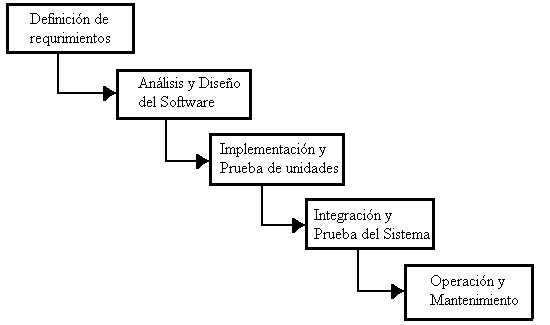
\includegraphics[scale=0.45]{M3_Modelo_Cascada}
	\caption{Modelo de proceso en cascada \cite{noauthor_archivo:modelo_nodate}}
	\label{fig:M3_Modelo_Cascada}
\end{figure}

\begin{figure}[!h]
	\centering
	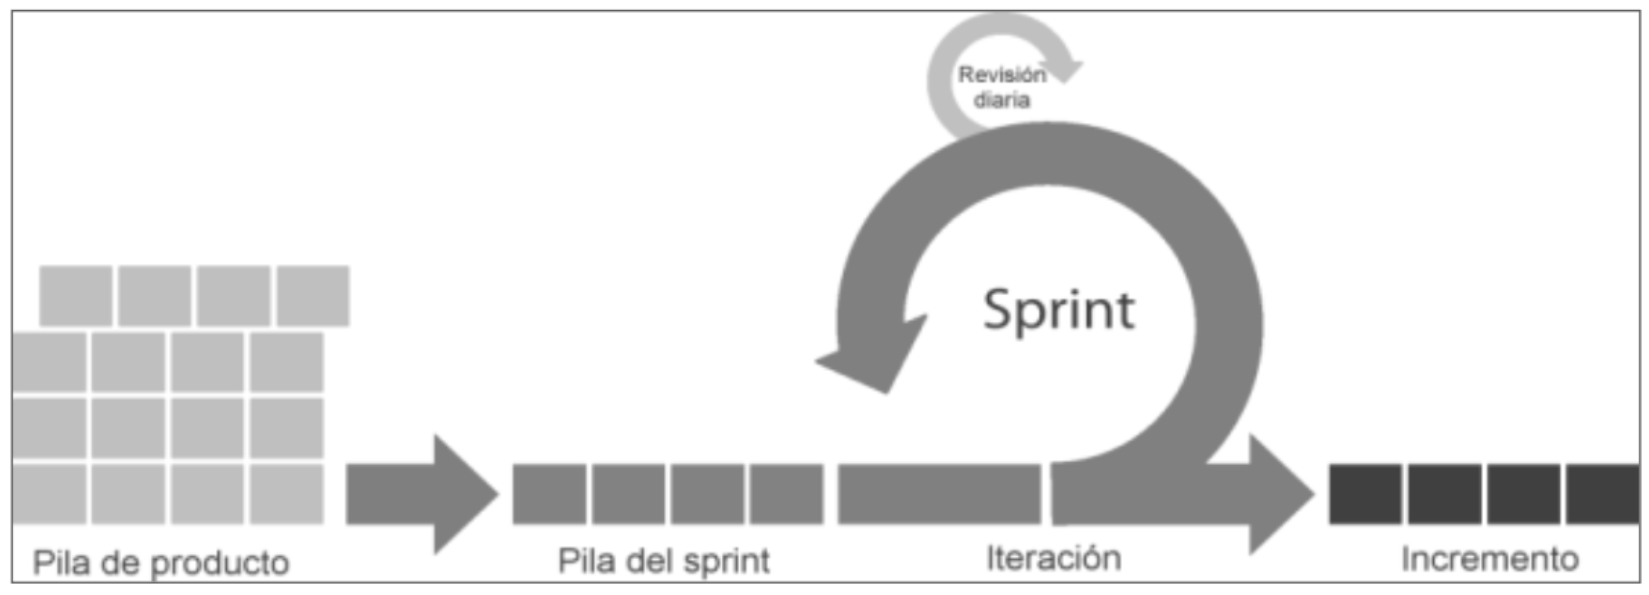
\includegraphics[scale=0.51]{M3_Scrum}
	\caption{Modelo de proceso incremental: Scrum \cite{noauthor_scrum_2019}}
	\label{fig:M3_Scrum}
\end{figure}

Sin embargo, estos modelos generales deben ser extendidos y adaptados para crear modelos más específicos. No existe un único proceso ideal para construir todos los productos software, ya que este proceso depende de la naturaleza del proyecto y de otros factores como el equipo de desarrollo, la estabilidad de los requisitos funcionales, la importancia de los requisitos no funcionales como escalabilidad, seguridad, licencias, lenguaje de programación, tipo de arquitectura de computación, etc. Todos estos factores hacen que el proceso sea bastante complejo y que se requiera un modelo diferente para cada proyecto.

\section{Repositorios y forjas de proyectos software}

%\todo Este párrafo está repetido en la introducción. Pero tiene que ser reducido, en este apartado se puede detallar más extensamente con alguna captura de pantalla  que ayude a describir las equivalentes en múltiples repositorios.
%\todo revisar

En el apartado anterior se habla sobre la complejidad de un proceso software y que este puede ser representado por modelos que ayudan a organizar las diferentes actividades. En este apartado se hablará sobre metodologías y herramientas que pueden ayudar en más de una actividad del ciclo de vida.

Los repositorios de código son espacios virtuales donde los equipos de desarrollo generan los artefactos colaborativos procedentes de las actividades de un proceso de desarrollo. Estas herramientas permiten a un equipo de desarrollo trabajar en paralelo, lo que en ingeniería del software es complicado ya que , por lo general, miembros del mismo equipo necesitan trabajar sobre el mismo fichero y esto genera conflictos. Normalmente estos espacios se encuentran en servidores por motivos de seguridad y facilitar a los miembros del equipo puedan acceder al repositorio.

Un buen repositorio no solo permite almacenar los artefactos generados por cada una de las actividades del ciclo de vida del software. Sino que, también, permite llevar un historial de cambios e incluso ayudará a entender el contexto de la aplicación: quién ha realizado los cambios y porqué, es decir que permite almacenar las interacciones entre los miembros del equipo. Para ello se utilizan distintos sistemas, dependiendo del artefacto generado: foros de comunicación, sistemas de control de versiones como \textit{Git}, sistemas de gestión de incidencias, sistemas de gestión de pruebas, sistemas de revisiones de calidad, sistemas de integración y despliegue continuo, etc. \cite{guemes-pena_emerging_2018}.

Además de estos repositorios han surgido en la última década forjas de proyectos software de fácil acceso tanto para proyectos empresariales como para proyectos open-source (SourceForge \footnote{\url{https://sourceforge.net/}}, GitHub \footnote{\url{https://github.com/}}, GitLab \footnote{\url{https://about.gitlab.com/}}, Bitbucket  \footnote{\url{https://bitbucket.org/}}). Este mismo proyecto está almacenado en un repositorio en GitLab\footnote{Enlace al repositorio del proyecto en GitLab: \url{https://gitlab.com/mlb0029/comparador-de-metricas-de-evolucion-en-repositorios-software}}, ver Fig. \ref{fig:M3_ProyectoGitLab}.

\imagen{M3_ProyectoGitLab}{Captura de este proyecto almacenado en GitLab}

Estas forjas suelen ofrecer servidores para almacenar repositorios e integran múltiples sistemas para dar soporte a los flujos de trabajo y registrar las interacciones entre los miembros del equipo, también ofrecen posibilidades para usar estos sistemas en un servidor particular. Además dan la posibilidad de extensión funcional con sistemas de terceros para gestionar otras actividades no soportadas directamente por la propia forja, como Travis CI \footnote{\url{https://travis-ci.org/}} para gestionar la integración continua o Codacy \footnote{\url{https://www.codacy.com/}} para gestionar las revisiones automáticas de calidad como se puede observar en la Fig. \ref{fig:M3_Codacy}. 

\imagen{M3_Codacy}{Revisión automática de calidad realizada con Codacy sobre este proyecto}

Actualmente estas forjas han tenido una gran aceptación entre la comunidad de desarrolladores y existen muchos desarrollos de software de tendencia que las utilizan. En la Fig. \ref{fig:M3-TrendForja} se aprecia como cambia la tendencia de utilización de dichas forjas en el tiempo. Actualmente la forja predominante es claramente GitHub pero se ve un incremento en el uso de GitLab.

\imagen{M3-TrendForja}{Comparativa de tendencia de búsqueda de Google desde 2004 con los términos de distintas forjas de proyectos software}

 Estas forjas de proyectos software están en constante evolución, tanto en sus estructuras estáticas como en sus interacciones dinámicas en los proyectos y se registran grandes conjuntos de datos difíciles de procesar. Sin embargo, las forjas de proyectos software proporcionan interfaces de programación específicas que permiten acceder a toda la información registrada.

El  desafío a la comunidad científica y empresarial  es constante mostrando un incremento en el interés en las aplicaciones de minería que mejoren sus sistemas de decisión \cite{guemes-pena_emerging_2018}. Estos datos que registran las forjas de repositorios pueden ser utilizados para mejorar estos sistemas de decisión en función de la evolución del proyecto.

\subsection{GitHub vs. GitLab}

%\todo introducir la sección
%\todo Usa la información de esta página \url{https://about.gitlab.com/devops-tools/github-vs-gitlab.html} para recoger las características de los repositorios 
%y su comparación.

Se ha hablado anteriormente de las forjas de repositorios como GitHub o GitLab y se puede observar en la Fig. \ref{fig:M3-TrendForja} la tendencia en el uso de diferentes forjas. Se observa como GitHub predomina sobre las demás y como crece el uso de GitLab. En esta sección se comparan los aspectos más relevantes de estas dos tendencias según los servicios que ofrecen.

\subsubsection{CI/CD - Continuous Integration/Continuous Delivery}
La integración y despliegue continuo son prácticas sirve para para construir, probar y, en caso de tratarse de una página web o una aplicación web, desplegar la aplicación una vez se combinen los cambios en el repositorio central, como se puede observar en Fig. \ref{fig:M3_CI-CD}. Ambos ofrecen la posibilidad de realizar este proceso mediante software de terceros como \textit{Travis CI}. Sin embargo, GitLab ofrece ejecutores o \textit{runners} propios para llevar este proceso desde GitLab. De hecho, en este trabajo con repositorio en GitLab se ha realizado este proceso definiendo un flujo de trabajos o \textit{pipeline} de la forma mostrada en la Fig. \ref{fig:M3_Pipeline}.

\imagen{M3_CI-CD}{CI/CD con GitLab \cite{noauthor_gitlab_nodate}}

\imagen{M3_Pipeline}{Flujo de trabajo para el proceso de CI/CD definido para este proyecto}

\subsubsection{Estadísticas e informes}
Ambos ofrecen estadísticas e informes sobre los datos que registran de los repositorios y pueden ser accedidos visualmente desde la web del repositorio o desde APIs de programación. Por ejemplo, las métricas que trabaja este proyecto se calculan a partir de datos proporcionados por estas APIs.

Algo que ofrece GitLab y no GitHub es la monitorización del rendimiento de las aplicaciones que se hayan desplegado.

\subsubsection{Importación y exportación de proyectos}
A diferencia de GitHub, GitLab ofrece la posibilidad de importar proyectos desde otras fuentes como GitHub, Bitbucket, Google Code, etc. También es posible exportar proyectos de GitLab a otros sistemas.

\subsubsection{Sistema de seguimiento de incidencias (issues)}
Ambos cuentan con un sistema de seguimiento de incidencias (\textit{issue tracking system} o \textit{issue tracker}), permiten crear plantillas para las incidencias, adornarlas con Markdown\footnote{Markdown es un lenguaje de marcado que facilita la aplicación de formato a un texto empleando una serie de caracteres de una forma especial\cite{lasso_que_2013}}, usar etiquetas o \textit{labels} para categorizarlas, asignarlas a uno o varios miembros del equipo y bloquearlas para que solo puedan comentarlas los miembros del equipo.

Sin embargo GitLab da un paso más y permite asignar peso a las tareas, crear \textit{milestones}, asignar fechas de vencimiento, marcar la incidencia como confidencial, relacionar incidencias, mover o copiar incidencias a otros proyectos, marcar incidencias duplicadas, exportarlas a CSV, entre otras cosas. Otros aspectos destacables de GitLab en cuanto a este tema son los gráficos Burndown de los milestones (ver Fig. \ref{fig:M3_BurndownChart}), acciones rápidas y la gestión de una lista de quehaceres (\textit{todos}) de un usuario cuándo a este se le asignan incidencias.

\imagen{M3_BurndownChart}{Ejemplo de gráfico burndown}

A diferencia de GitLab, GitHub mantiene un historial de cambios en los comentarios de una incidencia; permite asignar las incidencias a listas mediante ``drag and drop"; proporciona información útil al pasar el ratón por encima de elementos de la web como usuario, issues, etc.

\subsubsection{Wiki}
En ambas forjas es posible disponer de una wiki para el proyecto.

\subsubsection{Otros aspectos destacables}
\begin{itemize}
	\item GitHub permite repositorios 100\% binarios
	\item GitLab permite tener una instancia propia de GitLab en un servidor particular, lo que permite que se pueda gestionar software adicional dentro del servidor como sistemas de detección de intrusos o un monitor de rendimiento.
	\item GitLab permite elegir miembros del equipo como revisores de ``\textit{merge requests}''.
	\item El código de Gitlab EE puede ser modificado para ajustarlo a las necesidades de seguridad y desarrollo.
	\item Ambos incluyen APIs que permiten realizar aplicaciones que se integren con GitLab o GitHub. Esto ha sido clave para la realización de este proyecto, como se ha mencionado anteriormente.
	\item GitLab nos proporciona un  IDE\footnote{Integrated Development Environment - Entorno de Desarrollo Integrado } web para realizar modificaciones sobre el código desde el mismo GitLab, también incluye un terminal web para el IDE que permite, por ejemplo, compilar el código.
	\item Ambos permiten la integración con repositorios Maven\footnote{Software de gestión de proyectos software: \url{https://maven.apache.org/}}
\end{itemize}

\section{Calidad de un producto software}

El software debe tener la funcionalidad y el rendimiento requeridos por el usuario, además de ser mantenible, confiable, eficiente y fácil de utilizar.

La calidad de un producto de software no tiene que ver solo con que se cumplan todos los requisitos funcionales, sino también otros requerimientos no funcionales que no se incluyen en la especificación como los de mantenimiento, eficiencia y usabilidad.

%Comentar fig 25.3 - Ppales factores de la calidad de protducto software p561
Sommerville enumera en \textit{Software Engineering} \cite{sommerville_ingenierisoftware_2002} los principales factores que afectan a la calidad del producto, como se puede observar en la Fig. \ref{fig:M3-FactoresCalidad}:
\begin{itemize}
	\tightlist
	\item Calidad del proceso
	\item Tecnología de desarrollo
	\item Calidad del personal
	\item Costo, tiempo y duración
\end{itemize}
\begin{figure}[!h]
	\centering
	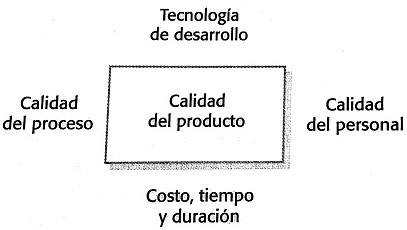
\includegraphics[scale=0.7]{M3-FactoresCalidad}
	\caption{Principales factores de calidad del producto de software\cite{sommerville_ingenierisoftware_2002}}\label{fig:M3-FactoresCalidad}
\end{figure}
\FloatBarrier

%Comentar fig 24.9 p549 relacion de metricas de proc y de prod

Para llegar a tener un software de calidad hay que tener en cuenta todos los factores mencionados anteriormente en cada una de las tres fases de la \textbf{administración de la calidad}: aseguramiento, planificación y control.

\begin{description}
	\item[Aseguramiento de la calidad.] Se encarga de establecer un marco de trabajo de procedimientos y estándares que guíen a construir software de calidad.
	\item[Planificación de la calidad.] Selección de procedimientos y estándares para un proyecto software especifico.
	\item[Control de la calidad.] La fase de control es la que se encarga de que el equipo de desarrollo cumpla los estándares y procedimientos definidos en el plan de calidad del proyecto. Esta fase puede realizarse mediante revisiones de calidad llevados a cabo por un grupo de personas y/o mediante un proceso automático llevado a cabo por algún programa.
\end{description}

%Comentar fg 24.1 p537 admin de calida en el proceso y desarrollo de software

\subsection{Control de la calidad: medición}

La fase de control de calidad es en la que se vigila que se sigan los procedimientos y estándares definidos en el plan de calidad. Pero estos podrían no ser adecuados o siempre pueden mejorar, por lo que en esta fase se puede valorar el mejorarlos como se puede observar en la Fig. \ref{fig:M3_CalidadProcesos}.

\imagen{M3_CalidadProcesos}{Calidad basada en procesos \cite{sommerville_ingenierisoftware_2002}}

Este proceso puede ser llevado a cabo mediante revisiones llevadas a cabo por un grupo de personas o por medio de programas que automaticen este proceso. El  desafío a la comunidad científica y empresarial es constante mostrando un incremento en el interés de aplicaciones que permiten  mejorar sus sistemas de decisión. Estas aplicaciones deberán llevar un control sobre el proceso y/o sobre el producto software y ese control se podrá realizar mediante un proceso de medición, esto ofrece una medida cuantitativa de los atributos del producto y del proceso software. 

La medición del software es un proceso en el cual se asignan valores numéricos o simbólicos a atributos de un producto o proceso software. Una métrica de software es una medida cuantitativa del grado en que un sistema, componente o proceso software posee un atributo dado. Las métricas son de control o de predicción. Las \textbf{métricas de control} se asocian al proceso de desarrollo del software, por ejemplo, la media de días que se tarda en cerrar una incidencia; y las \textbf{métricas de predicción} se asocian a productos software, por ejemplo, la complejidad ciclomática de una función. Y ambos tipos de métricas influyen en la toma de decisiones administrativas como se observa en la Fig. \ref{fig:M3-MetricasProcesoYProducto}. Los repositorios y las forjas facilitan la obtención de datos para este proceso de medición.

\imagen{M3-MetricasProcesoYProducto}{Métricas de control y métricas de predicción\cite{sommerville_ingenierisoftware_2002}}

Este proyecto se centra solo en la obtención de métricas de evolución que permitirán controlar y evaluar el proceso del desarrollo de un producto software. Por tanto se dejarán las métricas de predicción para otros trabajos y se detallará más sobre las de control en el siguiente apartado.

\subsection{Métricas de control: medición de la evolución o proceso de software}\label{sect:3_3_2_MetricasControl}

En la Fig. \ref{fig:M3-FactoresCalidad} se muestra la calidad de proceso como factor que afecta directamente a la calidad de producto. Parece lógico considerar como hipótesis que la calidad de un artefacto software tenga alguna relación con la manera en la que el equipo de desarrollo aplica las actividades del ciclo de vida del software dentro del repositorio. La validación empírica de estas  hipótesis ha abierto una nueva línea de aplicación con los conjuntos de datos que se pueden extraer de los repositorios gracias a interfaces de programación específicas que proporcionan estas forjas de repositorios y que permiten acceder a toda la información registrada.

Una plataforma de desarrollo colaborativo como GitLab puede presentar herramientas para controlar la evolución de un proyecto software. Por ejemplo un sistema de control de versiones (VCS - \textit{Version Control System}) como Git, un sistema de seguimiento de incidencias (\textit{Issue tracking system}), un sistema de integración continua (CI - \textit{Continuous Integration}), un sistema de despliegue continuo (CD - \textit{Continuous deploymen}t), etc.
Todas estas herramientas facilitan la comunicación entre los miembros de un equipo de desarrollo, ayudan a gestionar los cambios que producen cada uno de los miembros y proporcionan mediciones de proceso. Estas mediciones se pueden utilizar para obtener métricas de control que ayuden evaluar y mejorar la evolución del proyecto.

Las métricas de control que se utilizan en este proyecto provienen una Master Tesis titulada \textit{sPACE: Software Project Assessment in the Course of Evolution} \cite{ratzinger_space:_2007}. 
A continuación se describen las métricas que se implementan en este proyecto usando la plantilla de definición de la norma ISO 9126.

%\todo Cuando se ponen las fórmulas se puede utilizar el entorno matemático de Latex, mejora mucho la presentación.
%\todo Se puede utilizar el editor de Latex Web  \url{https://www.codecogs.com/latex/eqneditor.php?lang=es-es}
%\todo Un ejemplo de especificación  Sumatorio de (TCi-TCj) desde i=1, j=0 hasta i=NTC] / NTC. NTC
%\todo aplicando los entornos matemáticos $\frac{\sum_{i=1,j=0}^{NTC} TC_i - TC_j}{NTC}$
 
\textbf{\underline{I1 - Número total de issues (incidencias)}}

\begin{itemize}
	\item \textbf{Categoría}: Proceso de Orientación
	\item \textbf{Descripción}: Número total de issues creadas en el repositorio
	\item \textbf{Propósito}: ¿Cuántas issues se han definido en el repositorio?
	\item \textbf{Fórmula}: $NTI$. \textit{NTI = número total de issues}
	\item \textbf{Fuente de medición}: Proyecto en una plataforma de desarrollo colaborativo.
	\item \textbf{Interpretación}: $NTI \geq 0$. Valores bajos indican que no se utiliza un sistema de seguimiento de incidencias, podría ser porque el proyecto acaba de comenzar
	\item \textbf{Tipo de escala}: Absoluta
	\item \textbf{Tipo de medida}: \textit{NTI = Contador}
\end{itemize}

\textbf{\underline{I2 - Commits (cambios) por issue}}

\begin{itemize}
	\item \textbf{Categoría}: Proceso de Orientación
	\item \textbf{Descripción}: Número de commits por issue
	\item \textbf{Propósito}: ¿Cuál es el volumen medio de trabajo de las issues?
	\item \textbf{Fórmula}: $CI = \frac{NTC}{NTI}$. \textit{CI = Cambios por issue, NTC = Número total de commits, NTI = Numero total de issues}
	\item \textbf{Fuente de medición}: Proyecto en una plataforma de desarrollo colaborativo.
	\item \textbf{Interpretación}: $CI \geq 1$, Lo normal son valores altos. Si el valor es menor que uno significa que hay desarrollo sin documentar.
	\item \textbf{Tipo de escala}: Ratio 
	\item \textbf{Tipo de medida}: \textit{NTC, NTI = Contador}
\end{itemize}

\textbf{\underline{I3 - Porcentaje de issues cerradas}}

\begin{itemize}
	\item \textbf{Categoría}: Proceso de Orientación
	\item \textbf{Descripción}: Porcentaje de issues cerradas
	\item \textbf{Propósito}: ¿Qué porcentaje de issues definidas en el repositorio se han cerrado?
	\item \textbf{Fórmula}: $PIC = \frac{NTIC}{NTI}*100$. \textit{PIC = Porcentaje de issues cerradas, NTIC = Número total de issues cerradas, NTI = Numero total de issues}
	\item \textbf{Fuente de medición}: Proyecto en una plataforma de desarrollo colaborativo.
	\item \textbf{Interpretación}: $0 \leq PIC \leq 100$. Cuanto más alto mejor
	\item \textbf{Tipo de escala}: Ratio
	\item \textbf{Tipo de medida}: \textit{NTI, NTIC = Contador}
\end{itemize}

\textbf{\underline{TI1 - Media de días en cerrar una issue}}

\begin{itemize}
	\item \textbf{Categoría}: Constantes de tiempo
	\item \textbf{Descripción}:  Media de días en cerrar una issue
	\item \textbf{Propósito}: ¿Cuánto se suele tardar en cerrar una issue? 
	\item \textbf{Fórmula}: $MDCI = \frac{\sum_{i=0}^{NTIC}DCI_i}{NTIC}$. \textit{MDCI = Media de días en cerrar una issue, NTIC = Número total de issues cerradas, DCI = Días en cerrar la issue}
	\item \textbf{Fuente de medición}: Proyecto en una plataforma de desarrollo colaborativo.
	\item \textbf{Interpretación}: $MDCI \geq 0$. Cuanto más pequeño mejor. Si se siguen metodologías ágiles de desarrollo iterativo e incremental como SCRUM, la métrica debería indicar la duración del \textit{sprint} definido en la fase de planificación del proyecto. En SCRUM se recomiendan duraciones del \textit{sprint} de entre una y seis semanas, siendo recomendable que no exceda de un mes\cite{noauthor_scrum_2019}.
	\item \textbf{Tipo de escala}: Ratio
	\item \textbf{Tipo de medida}: \textit{NTI, NTIC = Contador}
\end{itemize}

\textbf{\underline{TC1 - Media de días entre commits}}

\begin{itemize}
	\item \textbf{Categoría}: Constantes de tiempo
	\item \textbf{Descripción}: Media de días que pasan entre dos commits consecutivos
	\item \textbf{Propósito}: ¿Cuántos días suelen pasar desde un commit hasta el siguiente?
	\item \textbf{Fórmula}: $MDC = \frac{\sum_{i=1}^{NTC} TC_i - TC_{i-1}}{NTC}$. $TC_i - TC_{i-1}$ en días; \textit{MDC = Media de días entre cambios, NTC = Número total de commits, TC = Tiempo de commit}
	%$MDEC = [Sumatorio de (TCi-TCj) desde i=1, j=0 hasta i=NTC] / NTC. NTC = Número total de commits, TC = Tiempo de Commit$ 
	\item \textbf{Fuente de medición}: Proyecto en una plataforma de desarrollo colaborativo.
	\item \textbf{Interpretación}: $MDEC \geq 0$. Cuanto más pequeño mejor. Se recomienda no superar los 5 días.
	\item \textbf{Tipo de escala}: Ratio
	\item \textbf{Tipo de medida}: \textit{NTC = Contador; TC = Tiempo}
\end{itemize}

\textbf{\underline{TC2 - Días entre primer y último commit}}

\begin{itemize}
	\item \textbf{Categoría}: Constantes de tiempo
	\item \textbf{Descripción}: Días transcurridos entre el primer y el ultimo commit 
	\item \textbf{Propósito}: ¿Cuantos días han pasado entre el primer y el último commit?
	\item \textbf{Fórmula}: $DEPUC = TC2- TC1$. $TC2- TC1$ en días;  \textit{DEPUC = Días entre primer y último commit, TC2 = Tiempo de último commit, TC1 = Tiempo de primer commit}
	\item \textbf{Fuente de medición}: Proyecto en una plataforma de desarrollo colaborativo.
	\item \textbf{Interpretación}: $DEPUC \geq 0$. Cuanto más alto, más tiempo lleva en desarrollo el proyecto. En procesos software empresariales se debería comparar con la estimación temporal de la fase de planificación. 
	\item \textbf{Tipo de escala}: Absoluta
	\item \textbf{Tipo de medida}: \textit{TC = Tiempo}
\end{itemize}

\textbf{\underline{TC3 - Ratio de actividad de commits por mes}}

\begin{itemize}
	\item \textbf{Categoría}: Constantes de tiempo
	\item \textbf{Descripción}: Muestra el número de commits relativos al número de meses
	\item \textbf{Propósito}:¿Cuál es el número medio de cambios por mes?
	\item \textbf{Fórmula}: $RCM = \frac{NTC}{NM}$. \textit{RCM = Ratio de cambios por mes, NTC = Número total de commits, NM = Número de meses que han pasado durante el desarrollo de la aplicación}
	\item \textbf{Fuente de medición}: Proyecto en una plataforma de desarrollo colaborativo.
	\item \textbf{Interpretación}: $RCM > 0$. Cuanto más alto mejor
	\item \textbf{Tipo de escala}: Ratio
	\item \textbf{Tipo de medida}: \textit{NTC = Contador}
\end{itemize}

\textbf{\underline{C1 - Cambios pico}}

\begin{itemize}
	\item \textbf{Categoría}: Constantes de tiempo
	\item \textbf{Descripción}: Número de commits en el mes que más commits se han realizado en relación con el número total de commits
	\item \textbf{Propósito}: ¿Cuál es la proporción de trabajo realizado en el mes con mayor número de cambios?
	\item \textbf{Fórmula}: $CP = \frac{NCMP}{NTC}$. \textit{CP = Cambios pico, NCMP = Número de commits en el mes pico, NTC = Número total de commits}
	\item \textbf{Fuente de medición}: Proyecto en una plataforma de desarrollo colaborativo.
	\item \textbf{Interpretación}: $0 \leq CCP \leq 1$. Mejor valores intermedios. Se recomienda no superar el 40\% del trabajo en un mes.
	\item \textbf{Tipo de escala}: Ratio
	\item \textbf{Tipo de medida}: \textit{NCMP, NTC = Contador}
\end{itemize}

\subsection{Framework de medición}\label{sect:3_3_3_FrameworkMedicion}

Para la implementación de las métricas se ha seguido la solución basada en frameworks propuesta en \textit{Soporte de Métricas con Independencia del Lenguaje para la Inferencia de Refactorizaciones} \cite{marticorena_soporte_2005}. El objetivo del \textit{framework} es la reutilización en la implementación del cálculo de métricas. Este diseño, mostrado en la Fig. \ref{fig:MCTMotorMetricas}, permite:

\begin{itemize}
	\item Facilitar el desarrollo de nuevas métricas
	\item Personalizar de los valores límite inferior y superior ya que estos pueden variar dependiendo del contexto en el que se calculen las métricas.
	\item Crear un grupo de configuraciones de métricas, de forma que se podrían calcular todas las métricas de ese grupo y almacenar los resultados en un colector de tipo \textit{MetricResult}
\end{itemize}

%Describir el diseño del motor de métricas, nombrar puntos de extensión
\imagen{MCTMotorMetricas}{Diagrama del framework para el cálculo de métricas con perfiles que almacena valores umbrales.}

En el diagrama UML de la Fig. \ref{fig:MCTMotorMetricas} se muestran las entidades principales del framework de medición y la relación entre ellas, especificando la navegabilidad y la multiplicidad. Las anotaciones en forma de flecha oscura especifican los patrones de diseño\citep{gamma_patrones_2002} aplicados en el framework.

Para crear una nueva métrica, esta deberá extender de la clase abstracta \textit{Metric} e implementar los métodos \textit{check()} y \textit{run()}. El método \textit{calculate()} de la clase \textit{Metric} utiliza el patrón de diseño \textbf{método plantilla}\footnote{\url{https://refactoring.guru/design-patterns/template-method}} que utiliza estos dos métodos, que deberán ser implementados por las clases concretas que hereden de \textit{Metric}. Un ejemplo de este método sería:

\begin{lstlisting}
...
Value calculate(Entity entity, 
		MetricConfiguration metricConfig, 
		MetricsResults metricsResults) 
{
	Value value;
	if(check(entity))
	{
		value = run(entity);
		metricsResults.addMeasure(new Measure(metricConfig, value));
	}
	return value;
}
...
\end{lstlisting}

Siendo \textit{entity} la entidad que se está midiendo, \textit{metricConfig} la configuración de valores limite que se está utilizando, \textit{metricsResults} el lugar donde se almacena el resultado y \textit{value} el valor medido en el método \textit{run()}. La plantilla establece que primero se comprueba que se pueda calcular la métrica y en ese caso se calcula y se añade a la coleción \textit{metricsResults}. 
Este método delega en las subclases el comportamiento de los métodos \textit{check()} y \textit{run()}. Además, almacena en el objeto colector \textit{metricsResults}, pasado como argumento, el valor medido para la configuración de la métrica para posibilitar el análisis y presentación de los resultados posteriores.

\textit{MetricConfiguration} toma el rol de decorador en el patrón de diseño \textbf{decorador}\footnote{\url{https://refactoring.guru/design-patterns/decorator}} que permite configurar los valores límite de las métricas. Implementa la misma interfaz que \textit{Metric}, \textit{IMetric}, y esta asociado a una métrica. Su método \textit{calculate()} simplemente llamará al método \textit{calculate()} de la métrica (\textit{Metric}) a la que esta asociada la configuración.

Un perfil de métricas agrupa un conjunto de configuraciones de métricas para un contexto dado, por ejemplo, para un conjunto de proyectos realizados por alumnos de la universidad en su realización del TFG. Se podría instanciar un \textit{MetricResult} para almacenar los resultados de toda esta colección de configuraciones de métricas y bastaría solo con recorrer el perfil usando el método \textit{calculate()} de cada configuración.

Este TFG ha adaptado este framework en el paquete ``motor de métricas'', y se han realizado unas pocas modificaciones. Las modificaciones más destacadas son:

\begin{itemize}
	\tightlist
	\item Se ha aplicado a las métricas concretas el patrón \textit{\textbf{Singleton}}\footnote{\url{https://refactoring.guru/design-patterns/singleton}}, que obliga a que solo haya una única instancia de cada métrica; y se ha aplicado el patrón \textit{\textbf{Método fábrica}}\footnote{\url{https://refactoring.guru/design-patterns/factory-method}} tal y como se muestra en la Fig. \ref{fig:M3_CambiosFrameworkMedicion1}, de forma que \textit{MetricConfiguration} no este asociada con la métrica en si, sino con una forma de obtenerla.\\
	La intencionalidad de esto es facilitar la persistencia de un perfil de métricas. Las métricas, se podrían ver como clases estáticas, no varían en tiempo de ejecución y solo debería haber una instancia de cada una de ellas. Por ello, al importar o exportar un perfil de métricas con su conjunto de configuraciones de métricas, estas configuraciones no deberían asociarse a la métrica, sino a la forma de acceder a la única instancia de esa métrica. 
	\item Se han añadido los métodos \textit{evaluate()} y \textit{getEvaluationFunction()} en la interfaz \textit{IMetric}, ver Fig. \ref{fig:M3_CambiosFrameworkMedicion2}.\\
	Esto permitirá interpretar y evaluar los valores medidos sobre los valores límite de la métrica o configuración de métrica. Por ejemplo, puede que para unas métricas un valor aceptable esté comprendido entre en valor límite superior y el valor límite inferior; y para oras un valor aceptable es aquel que supere el límite inferior.\\
	\textit{EvaluationFunction} es una interfaz funcional\footnote{
		\begin{itemize}
			\tightlist
			\item \url{https://docs.oracle.com/javase/8/docs/api/java/lang/FunctionalInterface.html}
			\item \url{https://docs.oracle.com/javase/8/docs/api/java/util/function/package-summary.html}
		\end{itemize}} 
	de tipo \textit{función}, recibe uno o más parámetros y devuelve un resultado. Este tipo de interfaces son posibles a partir de la versión 1.8 de Java \cite{noauthor_functionalinterface_nodate}.\\
	Esto permite definir los tipos de los parámetros y de retorno de una función que se puede almacenar en una variable. De esta forma se puede almacenar en una variable la forma en la que se puede evaluar la métrica.
\end{itemize}

\imagen{M3_CambiosFrameworkMedicion1}{Patrones ``singleton'' y ``método fábrica'' sobre el framework de medición}

\imagen{M3_CambiosFrameworkMedicion2}{Añadido al framework de medición la evaluación de métricas}